%-------------------------
% Resume in Latex
% Author : Sourabh Bajaj
% License : MIT
%------------------------

\documentclass[letterpaper,11pt]{article}

\usepackage{CJKutf8}
\usepackage{graphicx}
\usepackage{latexsym}
\usepackage[empty]{fullpage}
\usepackage{titlesec}
\usepackage{marvosym}
\usepackage[usenames,dvipsnames]{color}
\usepackage{verbatim}
\usepackage{enumitem}
\usepackage[hidelinks]{hyperref}
\usepackage{fancyhdr}
\usepackage[english]{babel}
\usepackage{tabularx}

\pagestyle{fancy}
\fancyhf{} % clear all header and footer fields
\fancyfoot{}
\renewcommand{\headrulewidth}{0pt}
\renewcommand{\footrulewidth}{0pt}

% Adjust margins
\addtolength{\oddsidemargin}{-0.5in}
\addtolength{\evensidemargin}{-0.5in}
\addtolength{\textwidth}{1in}
\addtolength{\topmargin}{-.5in}
\addtolength{\textheight}{1.0in}

\urlstyle{same}

\raggedbottom
\raggedright
\setlength{\tabcolsep}{0in}

% Sections formatting
\titleformat{\section}{
  \vspace{-4pt}\scshape\raggedright\large
}{}{0em}{}[\color{black}\titlerule \vspace{-5pt}]

%-------------------------
% Custom commands
\newcommand{\resumeItem}[2]{
  \item\small{
    \textbf{#1}{: #2 \vspace{-2pt}}
  }
}

\newcommand{\resumeSubheading}[4]{
  \vspace{-1pt}\item
    \begin{tabular*}{0.97\textwidth}[t]{l@{\extracolsep{\fill}}r}
      \textbf{#1} & #2 \\
      \textit{\small#3} & \textit{\small #4} \\
    \end{tabular*}\vspace{-5pt}
}

\newcommand{\resumeSubItem}[2]{\resumeItem{#1}{#2}\vspace{-4pt}}

\renewcommand{\labelitemii}{$\circ$}

\newcommand{\resumeSubHeadingListStart}{\begin{itemize}[leftmargin=*]}
\newcommand{\resumeSubHeadingListEnd}{\end{itemize}}
\newcommand{\resumeItemListStart}{\begin{itemize}}
\newcommand{\resumeItemListEnd}{\end{itemize}\vspace{-5pt}}

%-------------------------------------------
%%%%%   JAPANESE INPUT  %%%%%%%%%%%%%%%%%%%%

\newcommand{\ja}[1]{\begin{CJK}{UTF8}{ipxm}#1\end{CJK}}

%-------------------------------------------
%%%%%%  CV STARTS HERE  %%%%%%%%%%%%%%%%%%%%


\begin{document}

%----------HEADING-----------------
\begin{tabular*}{\textwidth}{l@{\extracolsep{\fill}}r}
  \textbf{\href{https://www.fosskers.ca/}{\Large Colin Woodbury}} & Email : \href{mailto:colin@fosskers.ca}{colin@fosskers.ca}\\
  \href{https://www.fosskers.ca/jp/cv}{https://www.fosskers.ca/jp/cv} & Mobile : +1-604-812-4532 \\
\end{tabular*}

\begin{figure}[h!]
  \centering
  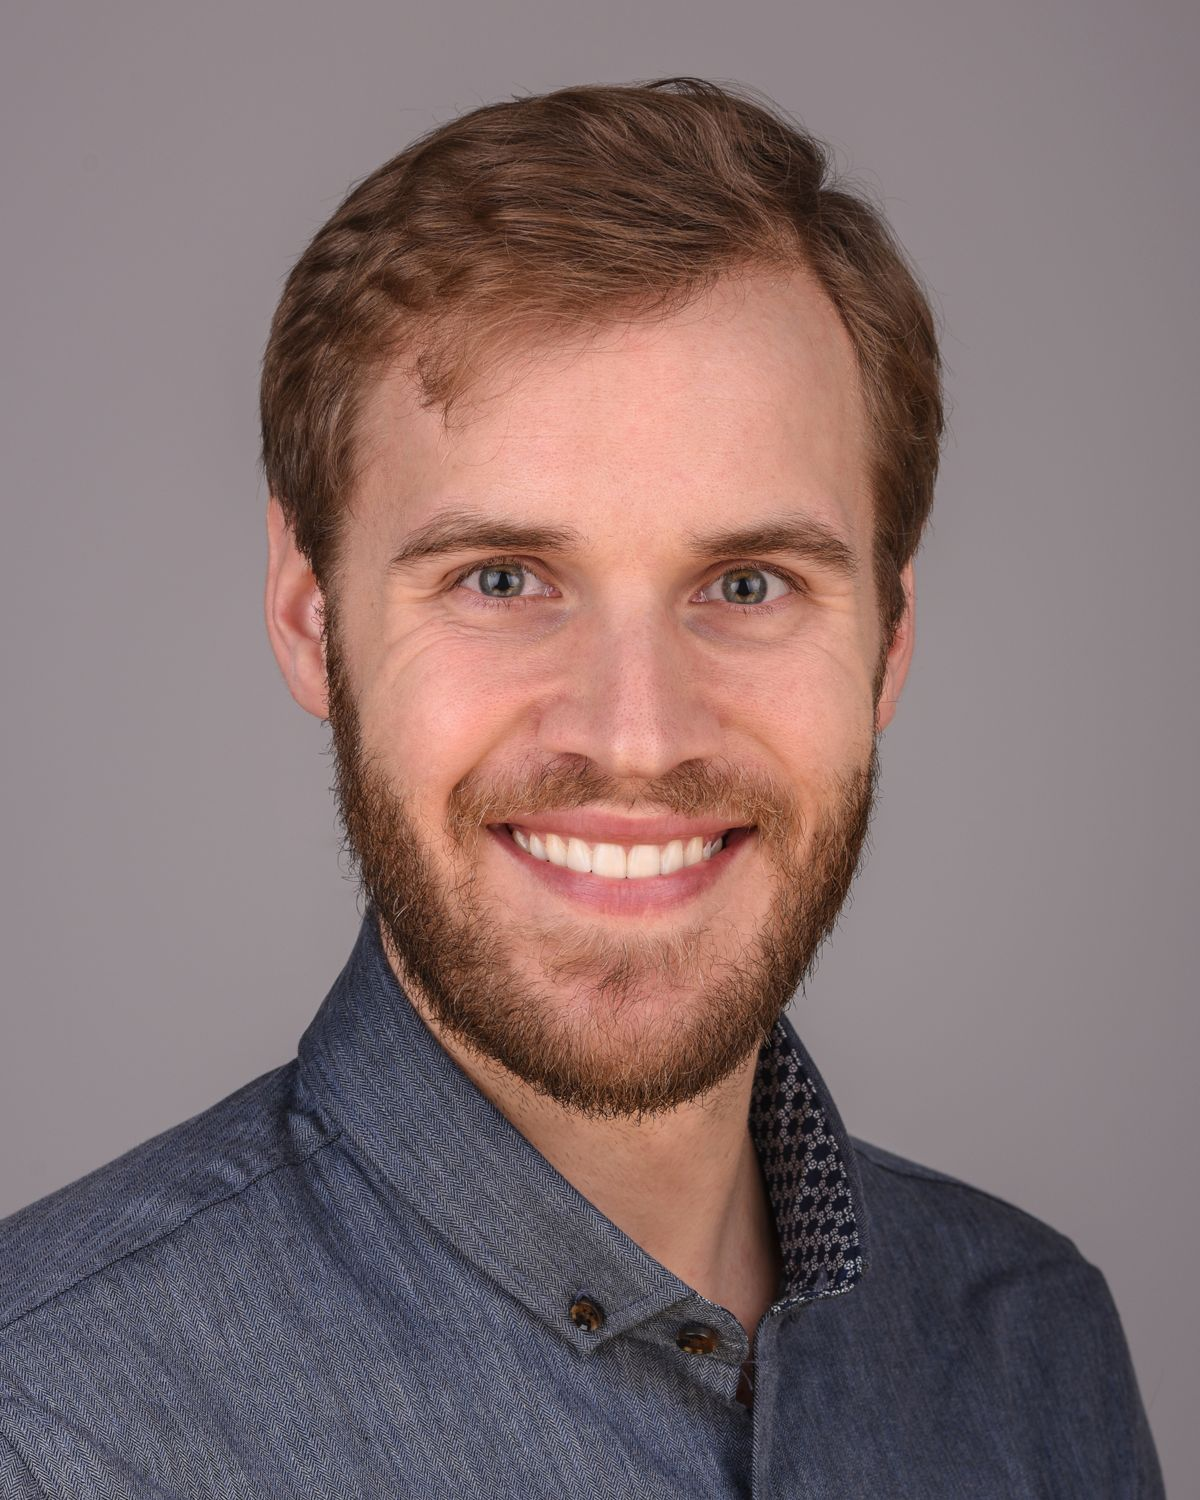
\includegraphics[width=0.25\linewidth]{colin.jpg}
\end{figure}

\begin{center}
  \ja{フルスタック開発者・オープンソース経験者} \\
  \ja{カナダの「生産的開発者ランキング」トップ20に選抜} \\
\end{center}

%--------PROGRAMMING SKILLS------------
\section{Skills}
\resumeSubHeadingListStart
\item{\textbf{Languages}{: Haskell, Purescript, Elm, Scala, Java, Python, C}}
\item{\textbf{Web Technologies}{: Terraform, AWS, Digital Ocean, Docker}}
\item{\textbf{Other}{: Linux, Git, SQL, MongoDB, Apache Spark, Nix}}
  \resumeSubHeadingListEnd


  %-------------------------------------------

%-----------EXPERIENCE-----------------
\section{Experience}
  \resumeSubHeadingListStart

    \resumeSubheading
      {Kadena}{New York, USA}
      {Haskell Software Developer}{2018 August - Present}
      \resumeItemListStart
        \resumeItem{Chainweb}
                   {Core developer of the Kadena Public Blockchain (Chainweb). Designed and implemented its Difficulty Adjustment algorithm. Pioneered Chainweb's mining algorithm and wrote its client, chainweb-miner.}

         \resumeItem{System Administration}
                    {Worked as the main system administrator for Kadena web servers. Managed servers on AWS with Terraform and NixOS.}
         \resumeItem{Documentation}
                    {Wrote extensive documentation in both Japanese and English.}
         \resumeItem{Public Speaking}
                    {Represented the company as a speaker at conferences in Japan, the USA, and Canada.}
      \resumeItemListEnd

    \resumeSubheading
        {Azavea}{Philadelphia, USA}
        {Scala Software Developer}{2016 May - 2017 December}
        \resumeItemListStart
          \resumeItem{GeoTrellis}{Open-source developer on the GeoTrellis project, a library suite for batch processing of geographic data using Apache Spark. Researched, designed, and implemented GIS algorithms.}
          \resumeItem{VectorPipe}{Wrote a library to process Vector Tile data through GeoTrellis.}
          %% \resumeItem{VectorTiles}{Wrote Haskell and Scala libraries that implement the Mapbox Vector Tiles spec.}
          \resumeItem{System Adminstration}{Used Docker and Terraform extensively to manage production systems on AWS.}
        \resumeItemListEnd

    \resumeSubheading
        {Adenda Media}{Vancouver, Canada}
        {Scala Software Developer}{2014 May - 2016 April}
        \resumeItemListStart
          \resumeItem{Adenda Backend}{Maintained and enhanced a Play + MySQL backend.}
          \resumeItem{Adenda Dashboard}{Extended a Twitter Bootstrap-based web application.}
          \resumeItem{Content Recommendation}{Implemented a content recommendation system using Apache Spark's MLlib.}
        \resumeItemListEnd

    \resumeSubheading
        {Sasebo Board of Education}{Sasebo, Japan}
        {English Teacher (ALT)}{2010 August - 2013 July}
        \resumeItemListStart
          \resumeItem{Middle School English}{Taught English to over a thousand Middle School students. Created lesson plans, supported Japanese colleagues, and helped grade tests.}
          \resumeItem{English Club}{Ran an English Club for students who wanted extra practice. Trained studets to participate in English speech contests.}
        \resumeItemListEnd


  \resumeSubHeadingListEnd

  %-----------PROJECTS-----------------
  \section{Open Source Projects}
  \resumeSubHeadingListStart
  \resumeSubItem{\href{https://github.com/aurapm/aura}{Aura}}{(Haskell) A package manager for Arch Linux.}
  \resumeSubItem{\href{https://github.com/kadena-community/bag-of-holding}{Bag of Holding}}{(Haskell) An ncurses-based terminal wallet for Chainweb.}
  \resumeSubItem{\href{https://github.com/fosskers/mapalgebra}{MapAlgebra}}{(Haskell) Library for efficient, polymorphic Map Algebra.}
  \resumeSubItem{\href{https://github.com/fosskers/kanji}{Kanji}}{(Haskell) Library for analysis of Japanese Kanji.}
  \resumeSubItem{\href{https://github.com/fosskers/hisp}{Hisp}}{(Haskell) A simple Lisp.}
  \resumeSubHeadingListEnd


%-----------EDUCATION-----------------
  \section{Education}
  \resumeSubHeadingListStart
  \resumeSubheading
      {Simon Fraser University}{Vancouver, Canada}
      {Post-Baccalaureate Diploma in Computing Science}{2013 September - 2016 April}
      \resumeSubheading
          {Saga University}{Saga, Japan}
          {SPACE Exchange Program for International Students}{2008 September - 2009 August}
          \resumeSubheading
              {University of Manitoba}{Winnipeg, Canada}
              {B.A. in Asian Studies - Minor in Computer Science}{2006 September - 2010 April}
              \resumeSubHeadingListEnd


%
\end{document}
